\section{Atividade 7}

\subsection{Análise Avançada do Lugar Geométrico das Raízes (LGR)}

A análise do Lugar Geométrico das Raízes (LGR) fornece insights essenciais sobre a estabilidade e as dinâmicas de resposta do sistema massa-mola-amortecedor, essencial para entender como variações nos parâmetros influenciam o sistema.

\subsection{Código Scilab para simular a resposta do sistema massa-mola-amortecedor}

O código Scilab detalhado abaixo estabelece os parâmetros do sistema, formula a função de transferência correspondente e visualiza o LGR, facilitando a identificação visual de características como estabilidade e comportamento assintótico.

\begin{lstlisting}[language=Scilab, caption=Código Scilab para simular o Lugar geométrico das raízes]
    // Definicao dos parametros
    M = 10;
    C = 7;
    K = 5;
    
    // Funcao de transferencia
    num = 1;  // Numerador e um polinomio constante
    den = [M, C, K];  // Coeficientes do denominador como vetor
    den_poly = poly(den, 's', 'coeff');  // Criacao do polinomio do denominador com os coeficientes
    
    // Sistema
    sys = syslin('c', num, den_poly);  // Cria o sistema com a funcao de transferencia
    
    // Configuracao da cor para o plot do LGR
    scf();  // Cria uma nova figura grafica
    clf();  // Limpa a figura
    sgrid();  // Adiciona uma grade ao grafico
    
    // Configuracoes de visualizacao de linha
    xset("line style", 4);  // Define o estilo da linha (ex: 4 - pontilhada)
    xset("thickness", 3);  // Define a espessura da linha
    xset("foreground", 5);  // Define a cor da linha (ex: 5 - vermelho)
    
    // Plotando o LGR com 50 pontos de discretizacao
    evans(sys, 50);  // Plota o LGR
    
    // Ajustes finais no grafico
    xtitle("Lugar Geometrico das Raizes (LGR)", "Re(s)", "Im(s)");  // Adiciona titulo e rotulos aos eixos
    
    // Anotacoes para polos
    polos = roots(den_poly);  // Calcula os polos do sistema
    for i = 1:size(polos, "r")
        // Adiciona anotacoes para cada polo no grafico
        xstring(real(polos(i)), imag(polos(i)), "Polo: "+string(polos(i)));
    end
    
    // Ajusta a visualizacao para um intervalo que inclua os polos
    zoom_rect([-1.8, -2.5, 0.2, 2.5]);
\end{lstlisting}

Este código é fundamental para visualizar como os polos do sistema variam com mudanças nos parâmetros, permitindo uma análise detalhada da estabilidade e do comportamento dinâmico do sistema massa-mola-amortecedor.

\begin{figure}[h]
    \centering
    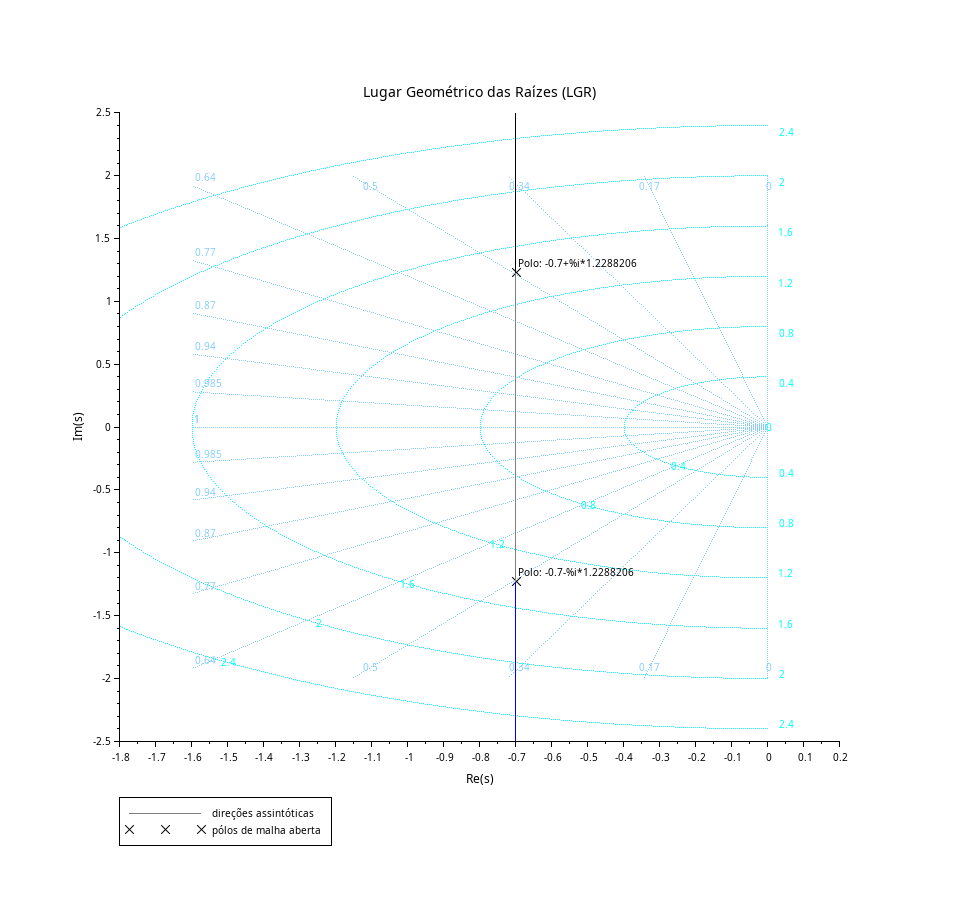
\includegraphics[width=0.8\textwidth]{atividades/7-atividade/assets/lgr.png}
    \caption{Lugar Geométrico das Raízes do sistema massa-mola-amortecedor.}
    \label{fig:LGR}
\end{figure}

Esta análise do Lugar Geométrico das Raízes (LGR) sugere uma tendência do sistema de manter a estabilidade diante de variações nos parâmetros, embora essa interpretação dependa de suposições sobre as condições de contorno e a natureza das mudanças paramétricas. As propriedades observadas nos pólos e nas assíntotas, particularmente sua simetria, fornecem indícios importantes para o design de sistemas de controle. No entanto, é essencial considerar que a visualização por meio do LGR oferece uma perspectiva limitada, que precisa ser complementada com outras análises dinâmicas para validar completamente a estabilidade e a eficácia do controle em cenários variados.

\begin{itemize}
    \item \textbf{Pólos e Simetria:}
          Os pólos do sistema, identificados claramente no LGR como \( s = -0.35 \pm j1.228\) (como mostrado na imagem com precisão real e imaginária), indicam uma resposta subamortecida do sistema devido ao posicionamento no semiplano esquerdo. A configuração destes pólos no semiplano esquerdo sugere uma estabilidade inerente sem oscilações não amortecidas.
          
    \item \textbf{Estabilidade e Assíntotas:}
          O sistema exibe duas assíntotas calculadas a partir da posição dos polos, indicando um movimento vertical dos pólos no plano complexo com o aumento do ganho do controlador. Estas assíntotas estão orientadas a \(90^\circ\) e \(-90^\circ\), garantindo que qualquer aumento nos parâmetros de controle mantenha a estabilidade desde que os pólos não cruzem o eixo imaginário.

    \item \textbf{Considerações sobre a Estabilidade:}
          A análise do LGR confirma a estabilidade do sistema com os pólos localizados estritamente no semiplano esquerdo. Entretanto, para garantir a validade dessa estabilidade sob diversas condições operacionais, sugere-se realizar análises adicionais como a de Nyquist ou Bode para avaliar a resposta do sistema frente a uma gama mais ampla de variações paramétricas.
\end{itemize}



